\documentclass[UTF8]{ctexart}
\usepackage{amsmath}
\usepackage{amssymb}
\usepackage{booktabs}
\usepackage{background}
\usepackage{caption,subcaption}
\usepackage{diagbox}
\usepackage{enumitem}
\usepackage{float}
\usepackage{fontspec}
%\usepackage{fourier}
\usepackage{geometry}
\usepackage{makecell}
\usepackage{mathptmx}
\usepackage{tasks}
\usepackage{tikz}
\usepackage{times}
\usetikzlibrary{arrows.meta, mindmap}
\usepackage{xcolor}

\geometry{a5paper, top=0.1cm, left=1cm, right=1cm, bottom=0.3cm, footskip=0.1cm}
\setCJKmainfont[BoldFont={汉仪文黑-85W},ItalicFont={方正苏新诗柳楷简体}]{汉仪文黑-55W}
\setfontfamily\Issue{Century Schoolbook}
\setfontfamily\Genshin{Genshin Teyvat Lingua Franca}
\newCJKfontfamily\TitleFont{思源宋体 CN Heavy}
\newfontfamily\timesnewroman{Times New Roman}
\captionsetup{font=small, labelfont=bf}
\setlist[itemize]{itemsep=0pt, parsep=0pt}
%\reversemarginpar

%\CTEXsetup[format = {\centering\bfseries\large}, beforeskip = 3pt, afterskip = 3pt]{section}
\CTEXsetup[format = {\color{cyan!50!black}\bfseries\large}]{subsection}

\settasks{label={\Alph*.}, label-format={\color{cyan!50!black}}}
\colorlet{darkcyan}{cyan!50!black}
\newcommand\Black[1]{\textcolor[gray]{0.3}{#1}}
\newcommand\Brown[1]{\textcolor[HTML]{998A4E}{#1}}
\newcommand\Emph[1]{\colorbox{green!10}{\textcolor{green!30!black}{#1}}}
\newcommand\Notes[1]{\textcolor{yellow!50!black}{\small #1}}
\newcommand\Example[1]{\textcolor{cyan!70!black}{\small #1}}


\newcommand\status[4]{\draw (#1 - 1,#2) circle (1) node{#3}; \draw (#1 + 1, #2) circle (1) node{#4};}
\renewcommand\d{\mathrm{d}}
\newcommand\Cov{\mathrm{Cov}}

\newcommand\IssueNumber{24}
\newcommand\Date{2024-4-18}
%\newcommand\Contributer{@金光日}
\newcommand\Subject{数据结构与算法}
\newcommand\Source{2022 考研 408 第 5 题}


\begin{document}
\backgroundsetup{contents=
\includegraphics{示例.png}, center, scale=1, angle=0, opacity=1}
\BgThispage
\begin{center}
%{\scriptsize\Issue \textcolor[HTML]{C8BA83}{\Genshin WEEKLY TIPS}}
\phantom{...}

{\Large\textcolor{brown!40!white}{\makebox[10cm][s]{\Genshin WEEKLY KNOWLEDGE TIPS}}}

\vspace{-2em}

{\Huge\bfseries\TitleFont \Black{知\ 识\ 小\ 料}}


\vspace{-0.1cm}
{\footnotesize \Brown{「电计 2203 班」周常规知识整理共享}}
\end{center}

\vspace{-0.5cm}


\begin{figure}[H]
\hspace{1cm}
\begin{minipage}[t]{0.3\textwidth}
\centering
    \Brown{\Genshin ISSUE}

    \vspace{-0.6cm}
    \Huge \Issue\slshape\bfseries\Black{\IssueNumber}
\end{minipage}
\hfill
\begin{minipage}[t]{0.35\textwidth}
\small
\centering
    \Brown{日期:\Date} \\
%\vspace{-0.1cm}
%    \Brown{贡献者:\Contributer} \\
\vspace{-0.1cm}
    \Brown{学科:\Subject} \\
\vspace{-0.1cm}
    \Brown{来源:\Source}
\end{minipage}
\hspace{0.8cm}
\end{figure}

{\color{cyan!50!black}
对任意给定的含 $n$($n>2$)个字符的有限集 $S$,用二叉树表示 $S$ 的哈夫曼编码集和定长编码集,分别得到二叉树 $T_1$ 和 $T_2$。下列叙述中,正确的是
{
\begin{tasks}[after-item-skip = 0pt]
    \task \color{cyan!50!black}  $T_1$ 与 $T_2$ 的结点数相同
    \task \color{cyan!50!black}  $T_1$ 的高度大于 $T_2$ 的高度
    \task \color{cyan!50!black}  出现频次不同的字符在 $T_1$ 中处于不同的层
    \task \color{cyan!50!black}  出现频次不同的字符在 $T_2$ 中处于相同的层
\end{tasks}
}}

哈夫曼树的特点就是变长编码,这与定长编码相对。举个例子:
\begin{figure}[htb]
\begin{minipage}[t]{.49\textwidth}
    \centering
    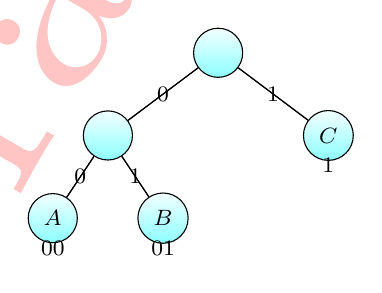
\begin{tikzpicture}
        \begin{scope}[mynode/.style = {circle, draw=black, top color=cyan!5!, bottom color=cyan!45!, font=\footnotesize},
        empty/.style = {rectangle, },
        level 1/.style = {sibling distance=40mm, level distance=15mm, mynode},
        level 2/.style = {sibling distance=20mm, mynode},
        level 3/.style = {sibling distance=10mm, mynode},
        every node/.style = {mynode}, scale = 0.7,]
            \node(rt){\phantom{X}} %root
            child { node(0){\phantom{X}}
                child{ node(00){$A$} }
                child{ node(01){$B$} }
            }
            child { node(1){$C$}};
        \end{scope}
        \begin{scope}[note/.style = {below, font=\footnotesize, outer sep = 5pt},
        path/.style = {font=\footnotesize, midway,}]
            \node[note] at (00) {00};
            \node[note] at (01) {01};
            \node[note] at (1) {1};
            \draw[] (rt) -- (0) node[path] {0};
            \draw[] (rt) -- (1) node[path] {1};
            \draw[] (0) -- (00) node[path] {0};
            \draw[] (0) -- (01) node[path] {1};
        \end{scope}
    \end{tikzpicture}
    \subcaption{哈夫曼编码 $T_1$}
\end{minipage}
\begin{minipage}[t]{.49\textwidth}
    \centering
    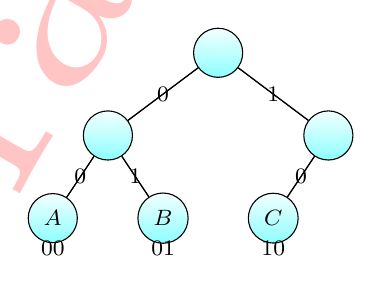
\begin{tikzpicture}
        \begin{scope}[mynode/.style = {circle, draw=black, top color=cyan!5!, bottom color=cyan!45!, font=\footnotesize},
        empty/.style = {rectangle, },
        level 1/.style = {sibling distance=40mm, level distance=15mm, mynode},
        level 2/.style = {sibling distance=20mm, mynode},
        level 3/.style = {sibling distance=10mm, mynode},
        every node/.style = {mynode}, scale = 0.7,]
            \node(rt){\phantom{X}} %root
            child { node(0){\phantom{X}}
                child{ node(00){$A$}}
                child{ node(01){$B$}}
            }
            child { node(1){\phantom{X}}
                child{ node(10){$C$}}
                child[missing]{ node(11){}}
            };
        \end{scope}
        \begin{scope}[note/.style = {below, font=\footnotesize, outer sep = 5pt},
        path/.style = {font=\footnotesize, midway,}]
            \node[note] at (00) {00};
            \node[note] at (01) {01};
            \node[note] at (10) {10};
            %\node[note] at (11) {11};
            \draw[] (rt) -- (0) node[path] {0};
            \draw[] (rt) -- (1) node[path] {1};
            \draw[] (0) -- (00) node[path] {0};
            \draw[] (0) -- (01) node[path] {1};
            \draw[] (1) -- (10) node[path] {0};
            %\draw[] (1) -- (11) node[path] {1};
        \end{scope}
    \end{tikzpicture}
    \subcaption{定长编码 $T_2$}
\end{minipage}
\end{figure}

在上图中,$C$ 的出现频率较高,$A,B$ 较低,但它们出现频率都可以不相同。

\begin{itemize}
    \item $T_1$ 和 $T_2$ 结点数不同,因为定长编码为了补齐层次,要比哈夫曼编码多一些结点。A 错误。
    \item $T_1$ 和 $T_2$ 高度相同。B 错误。
    \item 对于出现频次不同的字符,在 $T_1$ 中可能在同一层($A,B$)也可能在不同层($A,C$ 和 $B,C$),C 错误;在 $T_2$ 中必定处于同一层,而且都在叶结点,因为要保证编码长度相同,D 正确。
\end{itemize}

{\color{cyan!80!black} 【结论】D

【点评】本题考察了哈夫曼编码与定长编码的区别,明确哈夫曼树的缩短编码长度的意义,是解决此题的关键。
}

\end{document} 